\newpage
\section{Introduction}
\label{sec:introduction}
% state the learning objective 

The objective of this laboratory assignment is to choose an architecture of the Envelope Detector and Voltage Regulator circuits to build an AC/DC converter. We did this while paying attention to the merit of the project designed.\\
This merit is calculated exactly as the next equation:

\begin{equation} 
M = \frac{1}{cost*(ripple(V_{0}) + average(V_{0}-12) + 1e-6)}
\label{eq1}
\end{equation}

Being the cost the following:
\begin{itemize}
	\item cost = cost of resistors  + cost of capacitors + cost of diodes
	\item cost of resistors = 1 monetary unit (MU) per kOhm
	\item cost of capacitors = 1 MU/$\mu$F
	\item cost of diodes = 0.1 MU per diode
	
\end{itemize}

\begin{figure}[H] 
\centering
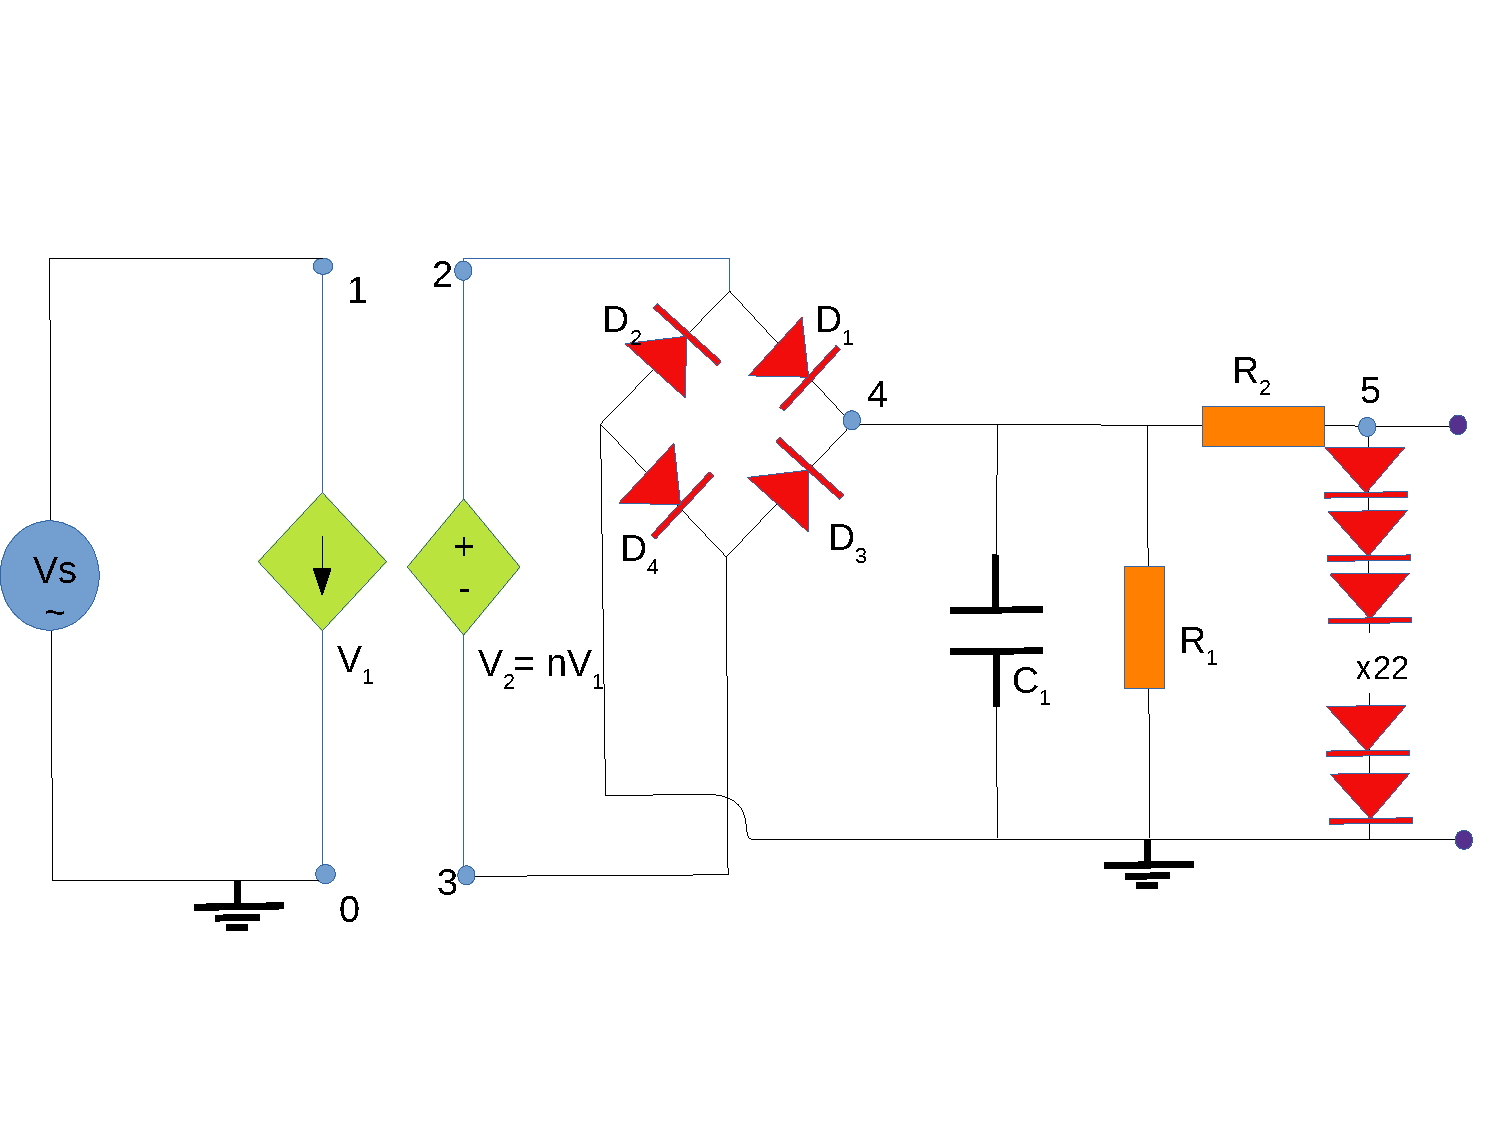
\includegraphics[width=\textwidth]{lab3draw.pdf} 
\caption{AC/DC Converter}
\label{fig:first}

\end{figure}

\begin{table}[H] \centering
\begin{tabular}{|
>{\columncolor[HTML]{FFCC67}}l |c|}
\hline
\multicolumn{2}{|l|}{\cellcolor[HTML]{EABD8B}Name - Value} \\ \hline
\input{../doc/Circuit_Values_tab}
\end{tabular}
\caption{Circuit Values}
\end{table}

To obtain the best values for the circuit, we've used the matlab simulink to optimize them for the best merit.

In Section~\ref{sec:analysis}, a theoretical analysis of the circuit is
presented. In Section~\ref{sec:simulation}, the circuit is analysed by
simulation, and the results are compared to the theoretical results obtained in
Section~\ref{sec:analysis}. The conclusions of this study are outlined in
Section~\ref{sec:conclusion}. \\


